\documentclass{article}
\usepackage{tikz}
\usetikzlibrary{shapes}
\usepackage{amsmath}
\usepackage{amssymb}
\begin{document}

\section{Procrastination MDP}
\label{sec:procrastination-mdp}
\vspace{1cm}
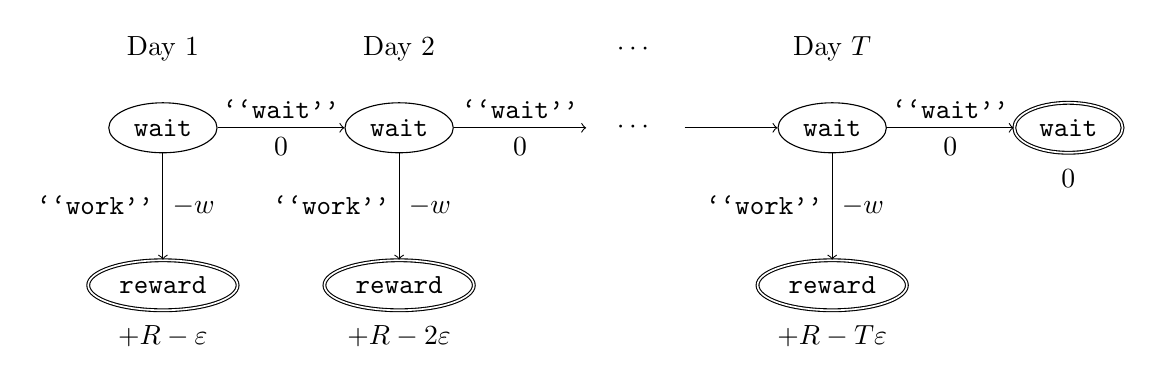
\begin{tikzpicture}
  \node (day1) at (0,3) {Day 1};
  \node (day2) at (3,3) {Day 2};
  \node (daysellipsis) at (6,3) {$\dotsb$};
  \node (dayt) at (8.5,3) {Day $T$};
  
  \node[draw, ellipse] (wait1) at (0,2) {\texttt{wait}};
  \node[draw, ellipse] (wait2) at (3,2) {\texttt{wait}};
  \node (waitellipsis-) at (5.5,2) {};
  \node (waitellipsis) at (6,2) {$\dotsb$};
  \node (waitellipsis+) at (6.5,2) {};
  \node[draw, ellipse] (wait3) at (8.5,2) {\texttt{wait}};
  \node[draw, double, ellipse] (wait4) at (11.5, 2) {\texttt{wait}};
  \node (utilityAtDeath) at (11.5, 1.35) {$0$};
  
  \node[draw, double, ellipse] (reward1) at (0,0) {\texttt{reward}};
  \node[draw, double, ellipse] (reward2) at (3,0) {\texttt{reward}};
  \node[draw, double, ellipse] (reward3) at (8.5,0) {\texttt{reward}};
  \node (utilityReward1) at (0, -0.65) {$+R - \varepsilon$};
  \node (utilityReward1) at (3, -0.65) {$+R - 2 \varepsilon$};
  \node (utilityReward1) at (8.5, -0.65) {$+R - T \varepsilon$};

  \draw[->] (wait1) -- node[above] {\texttt{``wait''}} node[ below] {$0$} (wait2);
  \draw[->] (wait2) -- node[above] {\texttt{``wait''}} node[ below] {$0$} (waitellipsis-);
  \draw[->] (waitellipsis+) -- (wait3);
  \draw[->] (wait3) -- node[above] {\texttt{``wait''}} node[ below] {$0$} (wait4);

  \draw[->] (wait1) -- node[left] {\texttt{``work''}} node[right] {$-w$} (reward1);
  \draw[->] (wait2) -- node[left] {\texttt{``work''}} node[right] {$-w$} (reward2);
  \draw[->] (wait3) -- node[left] {\texttt{``work''}} node[right] {$-w$} (reward3);

\end{tikzpicture}
\vspace{1cm}
\section{POMDP model}
\label{sec:pomdp-model}

\vspace{1cm}
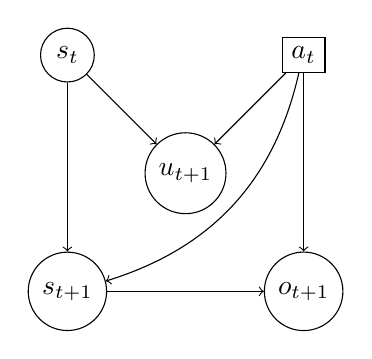
\begin{tikzpicture}
  \node[draw, circle] (st) at (0,3) {$s_t$};
  \node[draw, rectangle] (at) at (3,3) {$a_t$};
  \node[draw, circle] (ut) at (1.5,1.5) {$u_{t+1}$};
  \node[draw, circle] (st+1) at (0,0) {$s_{t+1}$};
  \node[draw, circle] (ot+1) at (3,0) {$o_{t+1}$};

  \path[->] (st) edge (st+1);
  \path[->] (at) edge (ut);
  \path[->] (st) edge (ut);
  \path[->] (at) edge[bend left] (st+1);
  \path[->] (st+1) edge (ot+1);
  \path[->] (at) edge (ot+1);
\end{tikzpicture}
\vspace{1cm}

\section{IRL Bandits}
\label{sec:irl-bandits}

\subsection{3c, first todo}
\label{sec:3c-first-todo}


\vspace{1cm}

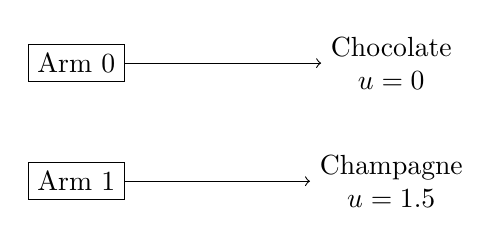
\begin{tikzpicture}
  \node[draw, rectangle] (arm0) at (0,1.5) {Arm 0};
  \node[draw, rectangle] (arm1) at (0,0) {Arm 1};
  \node[align=center] (prize1) at (4,0) {Champagne \\ $u = 1.5$};
  \node[align=center] (prize0) at (4,1.5) {Chocolate \\ $u = 0$};

  \path[->] (arm0) edge (prize0);
  \path[->] (arm1) edge (prize1);
\end{tikzpicture}

\end{document}
%%% Local Variables:
%%% mode: latex
%%% TeX-master: t
%%% End: